\begin{figure}
\centering

\subfigure[Example 1] {
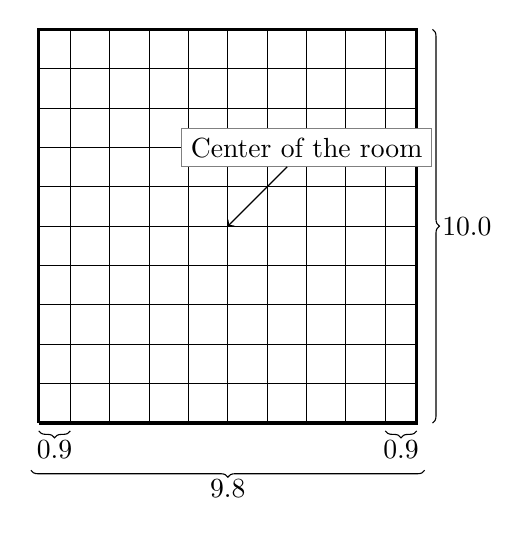
\begin{tikzpicture}[scale=.5]

\draw[step=1cm] (-4.8, -5) grid (4.8, 5);

\draw[very thick] (-4.8, -5) -- (4.8, -5) -- (4.8, 5) -- (-4.8, 5) -- (-4.8, -5);

\draw[decorate,decoration={brace,mirror}] (-4.8, -5.2) -- (-4, -5.2) node[midway,below] {0.9};
\draw[decorate,decoration={brace,mirror}] (4, -5.2) -- (4.8, -5.2) node[midway,below] {0.9};

\draw[decorate,decoration={brace,mirror}] (-5, -6.2) -- (5, -6.2) node[midway,below] {9.8};

\draw[decorate,decoration={brace,mirror}] (5.2, -5) -- (5.2, 5)  node [midway,right] {10.0};

\node (A) at (2,2) [rectangle,draw=black!50,fill=white] {Center of the room};
\draw[->] (A) -- (0,0);
\end{tikzpicture}
}
\subfigure[Example 2] {
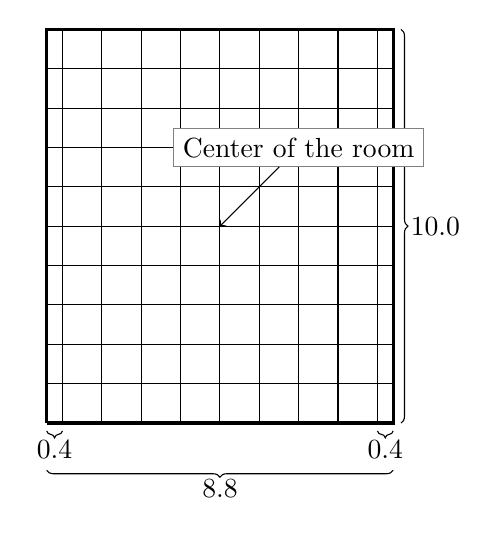
\begin{tikzpicture}[scale=.5]

\draw[step=1cm] (-4.4, -5) grid (4.4, 5);

\draw[very thick] (-4.4, -5) -- (4.4, -5) -- (4.4, 5) -- (-4.4, 5) -- (-4.4, -5);

\draw[decorate,decoration={brace,mirror}] (-4.4, -5.2) -- (-4, -5.2) node[midway,below] {0.4};
\draw[decorate,decoration={brace,mirror}] (4, -5.2) -- (4.4, -5.2) node[midway,below] {0.4};

\draw[decorate,decoration={brace,mirror}] (-4.4, -6.2) -- (4.4, -6.2) node[midway,below] {8.8};

\draw[decorate,decoration={brace,mirror}] (4.6, -5) -- (4.6, 5)  node [midway,right] {10.0};

\node (A) at (2,2) [rectangle,draw=black!50,fill=white] {Center of the room};
\draw[->] (A) -- (0,0);
\end{tikzpicture}
}
\caption{Examples of Floor Tiling}
\label{figure:floorTiling}
\end{figure}
